\section{Overall system architecture and services}
\begin{itemize}
	\item cf. \ref{fig:system-overview}
	\item \todo{highlight the differences between optimal (proposed) infrastructure and the implementation}
\end{itemize}

\begin{figure}[h]
	\centering
	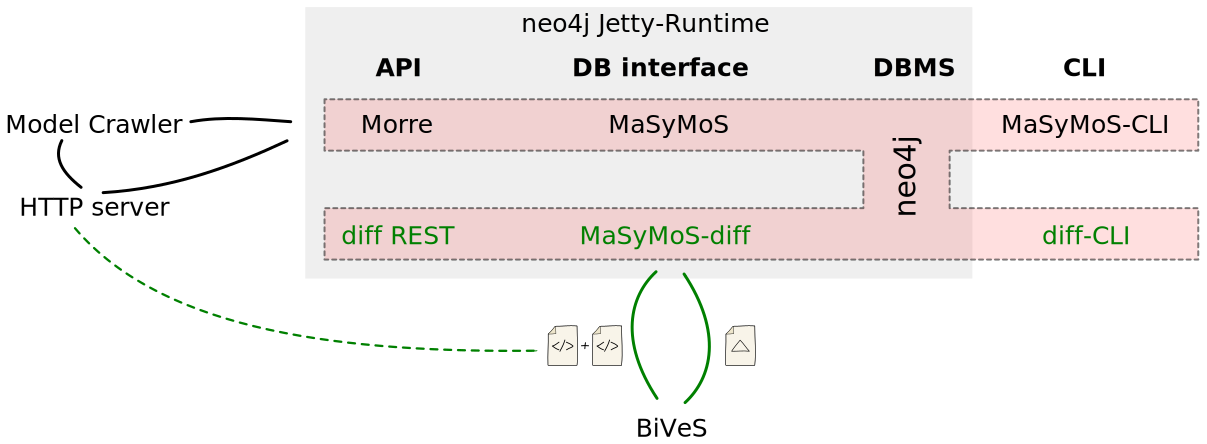
\includegraphics[width=\textwidth]{resources/system-overview-matrix.pdf}
	\caption{Infrastructure overview}
	\label{fig:system-overview}
\end{figure}

\section{Database model and storage decisions}
\begin{itemize}
\item extension to database model cf. \ref{fig:db-model}
	\subitem linking version
	\subitem storing differences
\item decisions on storage model
	\subitem storing each version full (no delta-storage)
	\subitem each version is aware to the search index
	\subitem diff still enables for analysis of changes
	\subitem higher storage consumption
\item extended storage model
\end{itemize}

% description of ER model
Figure \ref{fig:db-er-model} shows the proposed database schema as ER model. To reduce complexity and redundancy, for some entities only classes of higher hierarchy are modeled. E.g. a \texttt{DiffEntry} could be a \texttt{DiffInsert}, \texttt{DiffDelete}, \texttt{DiffModify} or \texttt{DiffMove}. Same applies for \texttt{ModelEntityType} and \texttt{ModelEntity}.
On the left hand side the model shows the existing structure, developed with \masymos. The entities and relations shown on the middle and right hand side shall be added in to process of prototype development.
\todo{Add color to the diagram, to ease explanation}

The schema is build around a \texttt{Diff} entity linking two \texttt{Document} entities, which are representing an (XML-)document containing a model. This entity does not necessarily need to span between two consecutive versions, but I decided for a standard setup it might be less useful to store differences between every possible combination of versions, since it would consume unreasonable amount of storage. Further are diffs concatable, so it does not take any computational effort to generate a diff for larger version steps out of consecutive diffs.

Every \texttt{Diff} entity links to multiple \texttt{DiffEntry} entities via the \texttt{has\_entry} relation. Each \texttt{DiffEntry} represents a difference detected by \bives \cite{Scharm2015}. Not modeled in the ER model is the differentiation between possible types of the diff (insert, delete, move, modify), which will be represented by using different additional label in \neoj.
Each \texttt{DiffEntry} links to at least on \texttt{ModleEntityType} or \texttt{ModelEntity} via either \texttt{old\_entity} or a \texttt{new\_entity}, depending on the type of the difference.



\begin{figure}
	\centering
	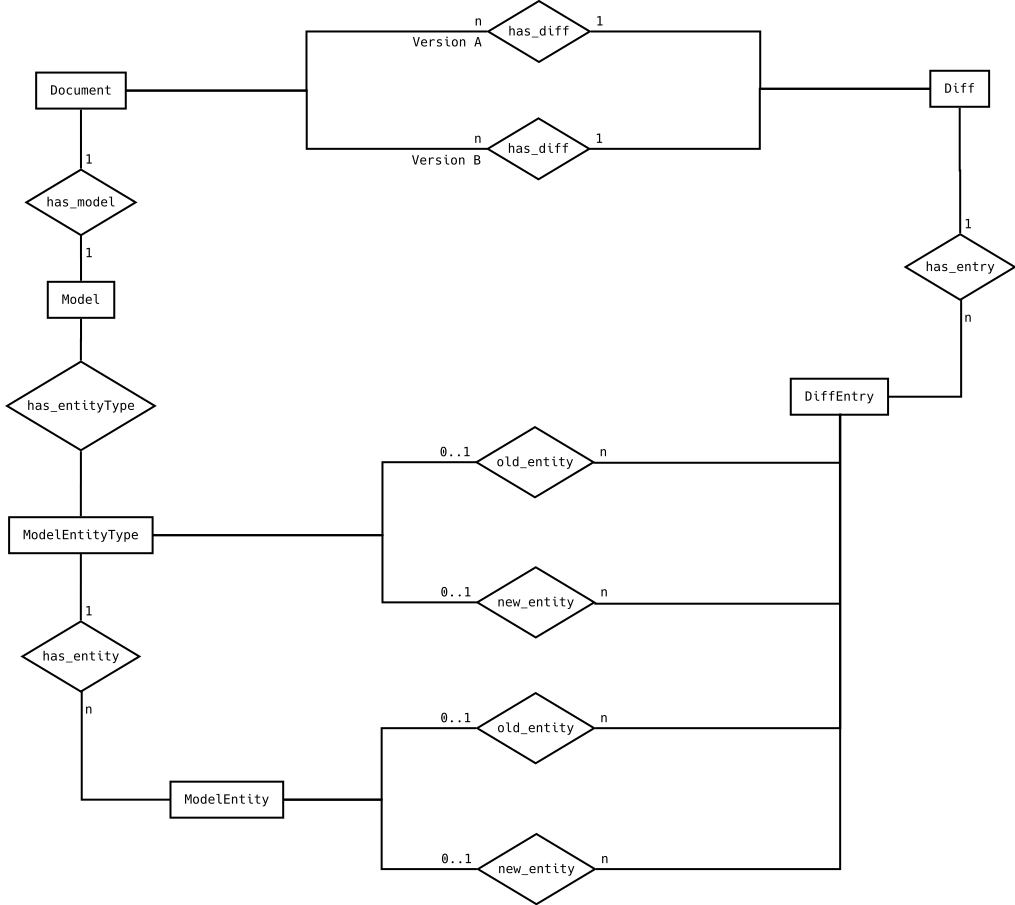
\includegraphics[width=\textwidth]{resources/db-concept-er.pdf}
	\caption{ER model of the proposed database schema}
	\label{fig:db-er-model}
\end{figure}

\begin{figure}[h]
	\includegraphics[width=\textwidth]{resources/db_structure.jpg}
	\caption{Proposed database structure}
	\label{fig:db-model}
\end{figure}
